% !TeX document-id = {759b9040-8a7f-4d09-8f16-a89e0a780c65}
%%% Magic comments for setting the correct parameters in compatible IDEs
% !TeX encoding = utf8
% !TeX program = pdflatex 
% !TeX spellcheck = en_US
% !BIB program = biber



\documentclass[notitlepage,english]{hgbreport}
%\usepackage{cmbright}
\usepackage{xfrac}
\usepackage{listings}
\usepackage[utf8]{inputenc}
\usepackage{cleveref}
\usepackage{wrapfig}
\usepackage{tcolorbox}

\usepackage{color, colortbl}
\definecolor{Gray}{gray}{0.925}
\renewcommand{\arraystretch}{1.15}


%acronyms
\newcommand{\Acronym}[1]{{#1}}
\newcommand{\LBP}{\Acronym{LBP}}
\newcommand{\SFM}{\Acronym{SFM}}

%-----
\newcommand{\Vertices}{\mathcal{V}}
\newcommand{\Edges}{\mathcal{N}}
\newcommand{\Graph}{\mathcal{G}}

%---------------------------------------------
\lstdefinelanguage{JavaScript}{
	keywords={typeof, new, true, false, catch, function, return, null, catch, switch, var, if, in, while, do, else, case, break},
	keywordstyle=\color{blue}\bfseries,
	ndkeywords={class, export, boolean, throw, implements, import, this},
	ndkeywordstyle=\color{darkgray}\bfseries,
	identifierstyle=\color{black},
	sensitive=false,
	comment=[l]{//},
	morecomment=[s]{/*}{*/},
	commentstyle=\color{purple}\ttfamily,
	stringstyle=\color{violet}\ttfamily,
	morestring=[b]',
	morestring=[b]"
}

\lstset{
	language=JavaScript,
	extendedchars=true,
	basicstyle=\footnotesize\ttfamily,
	showstringspaces=false,
	showspaces=false,
	numbers=left,
	numberstyle=\footnotesize,
	numbersep=9pt,
	tabsize=2,
	breaklines=true,
	showtabs=false,
	captionpos=b
}
%-----------------------------------------------

\graphicspath{{images/}}  % where the images at?
\bibliography{references}  % requires file 'references.bib'

%%%----------------------------------------------------------
\author{Giorgio Mariani}										% your name
\title{IM490 Depth-Map Recovery from RGB-video\\	% the name of the course or project
				\textbf{Project 1 Report}}	% or "Project Report"
\date{\today}
%%%----------------------------------------------------------


%%%----------------------------------------------------------
\begin{document}
%%%----------------------------------------------------------

\maketitle

\begin{abstract}\noindent
%This document is a simple template for a typical term or semester paper (lab/course report, ``Übungsbericht'', \etc) based on the \textsf{HagenbergThesis}\footnote{See \url{https://github.com/Digital-Media/HagenbergThesis} for the most current version
%and additional examples.
%This repository also provides a good introduction and useful hints for authoring academic texts with LaTeX.}
%The structure and chapter titles have been formulated to provide a good starting point for a typical \emph{project report}.
%This document uses the custom class \textsf{hgbreport} which is based on \latex's standard \textsf{report} 
%document class with \texttt{chapter} as the top structuring element. 
%If you wish to write this report in German you should substitute the line
\bigskip
\noindent
%Use the abstract to provide a short summary of the contents in the document.
\end{abstract}


%%%----------------------------------------------------------
\tableofcontents
%%%----------------------------------------------------------



%%%----------------------------------------------------------
\chapter{Aims and Context}
%%%----------------------------------------------------------

%Describe the initial goals and situation that lead to this project, requirements, as well as references to related work (\eg, \cite{Higham1998}).




\section{Introduction}
\label{sec:introduction}
% describe problem

The aim of this project is the implementation of the article \textit{"Consistent Depth Map Recovery from a Video Sequence"} \cite{Zhang2009}, by Zhang, Jia, Wong, and Bao and published in \textit{Transaction on Pattern Analysis and Machine Intelligence} (TPAMI).
%The article describes an algorithm which is able to generate a sequence of \emph{depth-maps} starting from an RGB-video.
The problem faced by Zhang et al. consists in the estimation of a sequence of \emph{depth-maps}\footnote{A \emph{depth-map} is an image in which each pixel maintains depth information.} starting from an RGB-video.
More precisely, given an image sequence representing a video of a static scene, the aim of the paper is to estimate a sequence of images with consistent depth values for each pixel and frame.
This depth values can then be  used for a variety of tasks, such as scene reconstruction and layer separation.
\begin{figure}[!h]
	\centering
	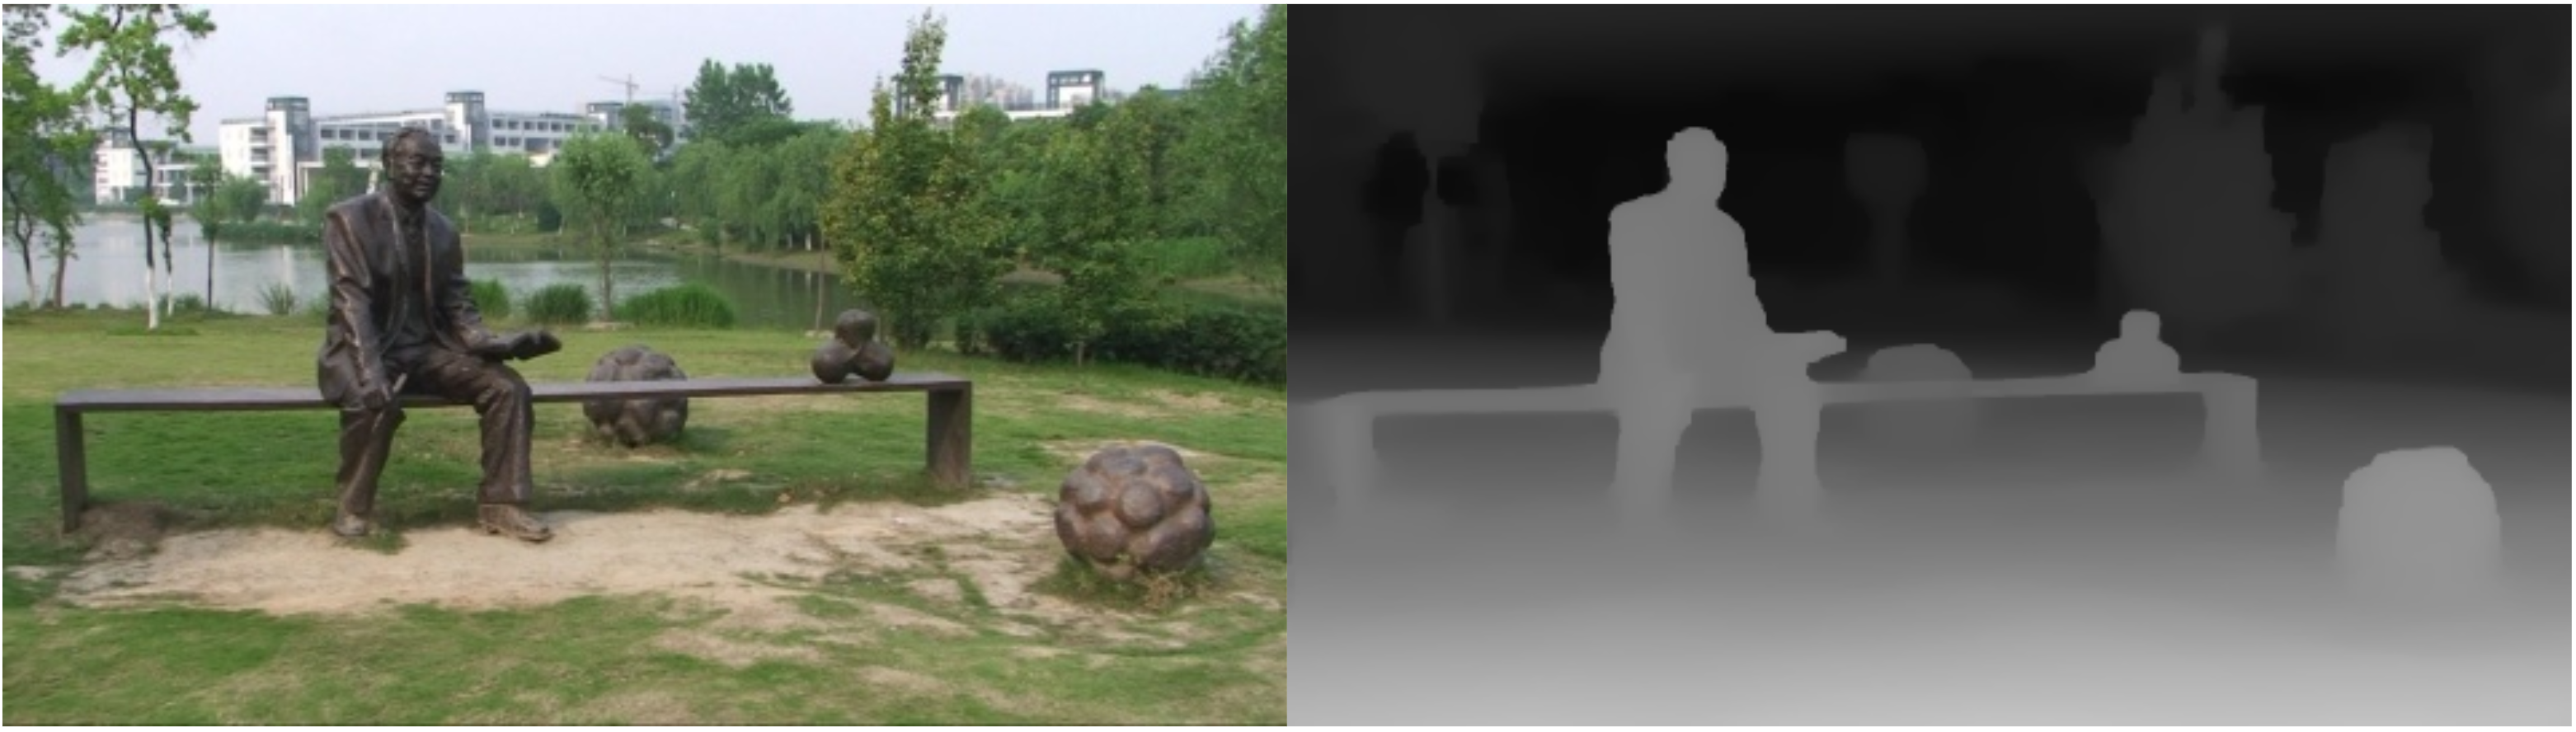
\includegraphics[width=.95\textwidth]{depthmap_example.png} %{CS0031}
	\caption{One of the estimated depth-map  obtained using \cite{Zhang2009} over a sequence of 200 images.}
\end{figure}

While a free implementation is available on the authors' website~\cite{CVGweb}, they do not offer its source code; hence, the reasons behind this project are to offer an open-source implementation of said article, and to offer didactic improvement for the project's author.

\section{Proposed Approach}
% overview of proposed solution
The approach proposed in the original article consists of four steps:
\begin{enumerate}
	\item Camera Parameter Estimation
	\item Depth-maps Initialization
	\item Depth-maps Bundle Optimization
	\item Depth-maps Space-Time Fusion
\end{enumerate}

\paragraph{Camera parameter estimation.} During this phase, the camera parameters (\ie \emph{position}, \emph{rotation}, and \emph{intrinsic matrix}) are estimated, using a \emph{Structure From Motion} (SFM) algorithm; unsurprisingly, the one used in the article is the same as the one described in \cite{Zhang2007}, with Zhang and Bao two of the article's authors.
\begin{figure}[!h]
	\centering
	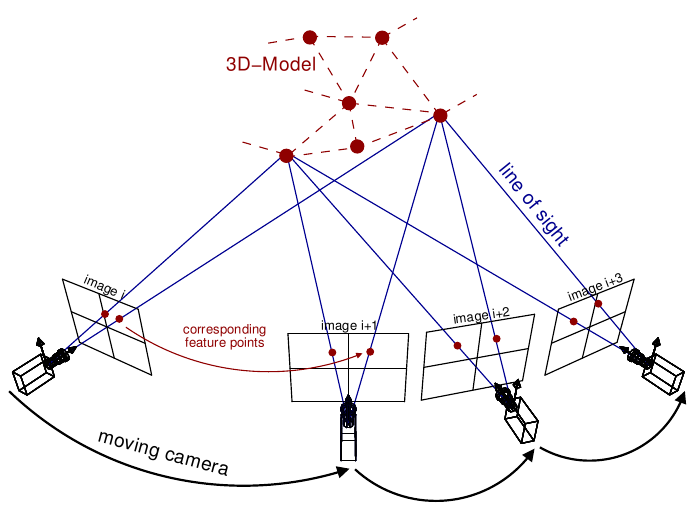
\includegraphics[width=.75\textwidth]{sfm.png} %{CS0031}
	\caption{SFM approach visualization}
\end{figure}

\paragraph{Depth-maps initialization.} 
For each frame in the video, a raw estimation of the corresponding depth-map is computed; this is achieved by minimizing a (per-frame) energy function whose parameters are the depth values to estimate.
These raw depth-maps are successively processed using a plane fitting algorithm: each image is divided into segments using \emph{mean-shift color segmentation} \cite{Comaniciu202}, these segments are then considered as a set of planes and fitted to the existing depth-maps raw values. The resulting images are the initialized depth-maps, ready to be used in the next step.

\paragraph{Depth-maps bundle optimization.} The depth-maps obtained during the initialization process are then refined by applying geometric coherence constraints. This refinement process iteratively elaborates the given raw data by minimizing an energy function similar to the one used in the previous step, but enriched with geometric-consistency constraints.

\paragraph{Depth-maps space-time fusion.} This is the final step of the process, and it is used to polish the results obtained from the previous steps and removing eventual remaining noise.

The estimated depth-map values are used to define a loss function  that can subsequently be optimized through the use of iterative \emph{Conjugate Gradient Method}, an optimization technique able to find approximate solution to energy-minimization  problems.
The designed loss function takes into consideration: \emph{spatial continuity} between already computed depth-values, the estimated depth-maps \emph{temporal coherence}, and consistency with the sparse points obtained by the SFM algorithm used to compute the camera parameters (see first step of the depth-maps estimation process).

 

\section{Related Work}
Since the proposed approach makes use of a variety of techniques, and it is relatively old (2009), the related work section is organized as follows:
\begin{enumerate}
	\item Previous work related to individual algorithms used in the proposed method.
	\item Work that makes use or improves the proposed solution. 
\end{enumerate}
\subsection{Previous Work}
[TODO]
\subsection{Future Work}
[TODO]

%CNN approaches




%%%----------------------------------------------------------
\chapter{Project Details}
%%%----------------------------------------------------------
%Describe important project steps, \eg, the rationale of the chosen architecture or technology stack, design decisions, algorithms used, interesting challenges faced on the way, lessons learned \etc


\section{The Architecture}
The systems is written using the \emph{Python Programming Language}; the reason behind this decision is the relative good performance that vectorized computation libraries can achieve on python, the flexibility and simplicity of the language, and the author's past experience with python libraries such as \textbf{NumPy} and \textbf{TensorFlow}, which makes the development less laborious.
%TODO say python version

\subsection{Dependencies and Third Party Libraries}
\paragraph{NumPy:} The main library used for computations in the project is the \textbf{NumPy} module: it is a set of function designed for intensive computing in vectorized fashion, similarly to the \textbf{MATLAB} programming language.

\paragraph{OpenCV:}
The \textbf{OpenCV} library (version 4.0.0) is also utilized in the project, using the official python bindings.
\textbf{OpenCV} offers real-time computer vision by exploiting (whenever possible) accelerated hardware, such as GPUs.
Unfortunately, the official bindings are available only for python 2.7.\textit{x} interpreters, forcing the author to use a compatible interpreter.
% TODO explain why OpenCV was chosen

%\subsection{Problems Encountered with OpenCV}



\section{Approach in Detail}
% in this section I will explain the implementation of each algorithm more in detail
 
 The goal of the system is to estimate a sequence of depth-maps $\hat D = D_0, \dots, D_n$, using a sequence of pictures $\hat I = I_0, \dots, I_n$ and camera paramet,ers: $\{R_i\}_{i=0..n}$, $\{T_i\}_{i=0..n}$, and $K$ (which are respectively  \emph{rotation}, \emph{position}, and \emph{intrinsic matrix} of the camera.)
 
 The estimated pixel $x$'s disparity\footnote{The disparity of a certain pixel $x$ correspond to the reciprocal of the pixel's depth ($\frac{1}{z_x}$), however, the terms \emph{depth} and \emph{disparity} are sometimes used interchangeably.} at time $t$ is noted with $D_t(x)$ ($d_x$ for short); the admissible disparity values are taken from the set $[d_{min}, d_{max}]$, subsequently to its quantization into $m$ uniformly spaced values $d_{min}=d_0, \dots, d_{m-1} = d_{max}$. This quantization process is necessary in order to execute the algorithms utilized by the system. This is especially true for \emph{Belief Propagation}, since it makes use of labels, not values in \R.

 
 
\subsection{Initialization Phase}\label{sec:init_phase}
During the initialization phase, for each frame in the input video, an initial depth-map is estimated; this estimation occurs with a two-step process: firstly, the depth-maps are initialized using a multi-view photo-consistency method and \emph{Loopy Belief Propagation} (\LBP) \cite{Felzenszwalb2006}. Then, \emph{mean-shift segmentation} and a plane fitting algorithm are used to refine the obtained results.

%\LBP{} is a dynamic programming algorithm that can be used to find good approximations for energy minimization problems defined over labeled graphs (see \cref{app:LBP} for more information).
%The \LBP{} algorithm requires the following inputs: a graph with vertices $\Vertices$ and edges $\Edges$, a set $D$ of possible vertex labels, a function $V$ that maps label pairs to real values and an array $U_x$ (for each vertex $x$) mapping labels to real values. The algorithms then  finds a label assignment $D_t(x)$, for each vertex $x$ in the graph, such that the energy function \ref{eq:lbp-example-energy} is locally minimized.

%Suppose to want to estimate the depth-map for an image $I$ in the sequence $I_0 ... I_m$, using \LBP; in such case, the graph nodes (the set $\Vertices$) are the image's pixels, furthermore, each node has as neighborhood the (at most) four adjacent pixels.
%The labels (set $D$) represents the depth values that should be estimated. The edge function $V$ can be defined as
%$$V(D_t(x), D_t(y)) = \lambda(x,y)\cdot\min\{|D_t(x) - D_t(y)|, \eta\}$$
%with $\eta$ a constant value and $\lambda$ a smoothness weight proportional to the disparity in color of an edge (\ie{} the more the $I(x)$ is distant from $I(y)$ the smaller $\lambda(x,y)$ is). This definition for $V$ entice the difference between adjacent to not be more smooth, especially if said adjacent vertices are similar in color, and it is compliant with the \LBP{} requirements\footnote{Only a specific class of edge functions can be used for \LBP.}.

%Finally, each $U_x(d)$ value is computed by projecting the pixel position  for a particular time instant $t$, using the depth-label $d$ and the camera parameters. The difference between the original pixel position color and the projected position color at time $t$ is then used to describe the likeness that $d$ is an acceptable depth-value for the pixel $x$. Summing and normalizing these differences for all time instants $t$ gives the actual value $U_x(d)$.

The initial depth-maps estimation process works by minimizing the energy function $E_{init}$, which is defined as
\begin{equation}
\label{eq:init_energy}
E_{init}(\hat D) = \sum_{t} \left(E_{data}^t(D_t) + E_{smooth}(D_t)\right).
\end{equation}
The variable $t$ iterates over the video sequence frames, while the term $E^t_{data}$ indicates how much photo-consistent is the input depth-map $D_t$. Finally, $E_{smooth}^t$ indicates how smooth\footnote{That is, how much difference there is between adjacent disparities.} the $D_t$ depth-map is.

\paragraph{Energy Data Term.}
The term $E_{data}^t(D_t)$ is defined in terms of \emph{disparity likelihood}, noted as $L_{init}$ and defined as
$$L_{init}(x, d) = \sum_{t'} p_c(x,d,t,t').$$
This likelihood is used to the describe the photo-consistency of a certain disparity value $d$; furthermore, the function $p_c(x,d,t,t')$ describes how much the pixel $x$, using depth $1/d$, is photo-consistent. $p_c$ is expressed as
$$p_c(x,d,t,t') = \frac{\sigma_c}{\sigma_c + \Vert I_t(x) - I_{t'}(l_{t,t'}(x,d))\rVert},$$
with $\sigma_c$ a constant value and $l_{t,t'}(x,d)$ the projection of pixel $x$ (taken from $I_t$) at time $t'$, using disparity $d$.
Finally, 
\begin{equation}\label{eq:init_energy_data}
E_{data}^t(D_t) = \sum_{x}1 -  u(x) \cdot L_{init}(x,D_t(x)),
\end{equation}
with $u(x)$ a normalization factor, such that the maximum value of the likelihood is 1; more precisely, it is true that $\max_{d} \{u(x)\cdot L_x(d)\} = 1$ (\ie the normalization is applied only with respect of the disparity value $d$ and not the pixel $x$).

\paragraph{Energy Smoothness Term.}
The smoothness term $E_{smooth}(D_t)$ is used to impose a smoother gradient during estimation.
This smoothness imposing strategy assigns an higher cost if two adjacent pixels have starkly different disparity-labels.
This label difference is measured using the function
$$\rho(d_x,d_y) = \min\{|d_x-d_y|, \eta\}.$$
The term $\eta$ is a real constant positive value, and it represents the upper limit of this smoothness imposing approach: after $\eta$ the distance between two labels does not matter during the energy minimization.

The value $\rho(\cdot)$ is then weighted using an adaptive smoothness weight $\lambda(x,y)$, which encodes changes of color between the adjacent pixels $x$, $y$: if $x$ and $y$ have strongly different colors in $I_t$ then the disparity smoothness requirement should be less strict, since they are less likely to be in a contiguous three-dimensional area. This is expressed as 
$$\lambda(x,y) = w_s\cdot \frac{u_\lambda(x)}{|| I_t(x) - I_t(y)|| + \epsilon},$$
with $w_s$ a constant real positive value and $u_{\lambda}(x)$ a normalization factor
$$
	u_{\lambda}(x) = {|N(x)|}\big/{\sum_{y'\in N(x)} \frac{1}{||I_t(x) - I_t(y')||+\epsilon}}.
$$
The smoothness term definition is then
\begin{equation}
	E_{smooth}(D_t) = \sum_x \sum_{y\in N(x)} \lambda(x,y)\cdot \rho(D_t(x),D_t(y)).
\end{equation}

\paragraph{Minimization.}
$E_{init}$ is then minimized using \LBP{}, process which requires a-priori the computation of an $h\times w\times m$ bi-dimensional table that stores the value
$$1-u(x)\cdot L_{init}(x,d)$$ for each possible disparity-values $d$ and pixel $x$. To see how this table is computed look at \cref{sec:init_phase_alg}.




\paragraph{Color Segmentation Refinement.}
Finally, using \emph{mean-shift segmentation}, it is possible to divide an image $I_t$ into different segments, which are then fitted to the initial estimation $D_t$:
\begin{enumerate}
\item First, the depth of the plane is selected by using the disparity that minimizes \cref{eq:init_energy}. The slope is assumed to be 0 during the fitting process.
\item Then, by using \emph{Levenberg-Marquardt algorithm}, the planes' slopes are estimated.
\end{enumerate}
These output planes represent the new refined depth-map, and are ready to be processed by the next phase of the algorithm.%(or used independently if precision is not that important)

\subsection{Initialization Phase - Algorithm}\label{sec:init_phase_alg}
In order to minimize the energy function described in \cref{eq:init_energy}, the \LBP{} algorithm (see \cref{app:LBP} for more information) is used.
\LBP{} is a dynamic programming algorithm which can be used to find good approximations for energy minimization problems defined over labeled graphs.
For the depth-map recovery problem, the image is expressed as a grid graph (with each node representing a pixel and having at most four adjacent nodes), and the possible labels are the disparity values $d_0\dots d_{m-1}$. Therefore, an assignment of these labels over the graph can be thought of as a depth-map.

In order to work, the \LBP{} algorithm requires some data, specifically, it requires, for each pixel $x$ and disparity value $d$, the cost of assigning to $x$ the disparity $d$: this is expressed as $ 1- u(x)\cdot L_{init}(x,d)$ (see \cref{eq:init_energy_data}). Thus, it is necessary to compute a table able to store such information. 
The computation of this table is performed by the function \texttt{compute\_energy\_data}, which evaluates $1-u(x)\cdot L(d)$ for each possible pixel $x$ and disparity value $d$. 
\begin{algorithm}[H]
	\caption{\texttt{compute\_energy\_data\_init }(camera, $t$, $\hat I$)}
	\label{alg:energy_data_init}
\begin{algorithmic}[1]
	\State h $\leftarrow$ camera.height
	\State w $\leftarrow$ camera.width
	\State $I_t \leftarrow \hat I[ t ]$
	\State
	\State $x^h \leftarrow$ \texttt{homogeneous\_coordinate\_grid}(h,w)
	\State create table $L$ with $m\times h \times w$ elements, initialized with zero
	%\State L $\leftarrow$ $m\times h \times w$ table, initialized with zero
	\State
	\For {$t'\leftarrow 0\dots n$}
		\State $I_{t'} \leftarrow \hat I[ t' ]$
		\For {${level}\leftarrow 0\dots m$}
		\State create matrix $D$ with $h \times w$ elements, initialized with value $d_{level}$
		%\State $\mathrm{d}[i,j] \leftarrow \mathrm{depth\_values}[level]$, $\forall i,\forall j$
		\State $x'^h\leftarrow$ \texttt{conjugate\_coordinates}(camera, $t$,  $t'$, $x^h$, $D$)
		\State $I^r_{t'} \leftarrow$ \texttt{remap}($I_{t'}$, $x'^h$)
		%\State color\_diff $\leftarrow$ \texttt{L2\_norm}($I_t - I^r_{t'}$)
		\State
		\State $p_c \leftarrow$  $\sigma_c$ / $(\sigma_c +$ \texttt{L2\_norm($I_t - I^r_{t'}$)})
		\State $L[level] \leftarrow L[level] + p_c$
		\EndFor
	\EndFor
	\State
	\State $u \leftarrow$ $1$/ \texttt{max\_reduce}($L$, 0)
	\State \Return $1 - u\cdot L$
\end{algorithmic}
\end{algorithm}
\begin{figure}[!h]
	\centering
	\begin{tabular}{|l  l|}\hline\hline
		\textbf{variable}&\textbf{shape}\\
		$x^h$, $x'^h$&  $3\times h\times w$\\
		$D$ & $h\times w$\\
		$I_t$, $I_{t'}$, $I^p_{t'}$&$h\times w$\\
		$L$&$m\times h \times w$\\
		$p_c$, $u$&$h\times w$\\\hline\hline
	\end{tabular}
	\caption{Shapes of the variables in \cref{alg:energy_data_init} }
\end{figure}

The procedure \texttt{homogeneous\_coordinate\_grid}(h,w) produces a multi-dimensional array $x^h$ which stores a grid of homogeneous coordinates, such that the first axis represent the coordinate itself, \ie
\begin{align*}
	x^h[0,i,j] &= i\\
	x^h[1,i,j] &= j\\
	x^h[2,i,j] &= 1
\end{align*}

The coordinates assume integer values between $0$ to $h$ (excluded) for the second axis (that is, value $i$ in above equation) and between $0$ and $w$ (excluded) for the third axis (value $j$). Consequently, $x^h$'s shape is $3\times h \times w$.

The procedure \texttt{conjugate\_coordinates}($camera$, $t$, $t'$, $x^h$, $D$) computes, for each coordinate in $x^h$, the respective conjugate coordinate at time $t$ if the depth stored in $D$ is used. The implementation of this procedure is explained in \cref{app:conjugate_pixel}.

The procedure $I'\leftarrow$ \texttt{remap}($I$, $map$) is used to transform the input image $I$ using a certain mapping $m$ (which should have shape $h\times w\times 2$) such that
$$I'[x,y] = I[map[x,y]].$$
The reader should note that in \cref{alg:energy_data_init} there is an abuse of notation, since the variable $x'^h$ (which assumes role of the argument $map$ in the function call) has shape $3\times h \times w$ instead of the required $h\times w \times 2$; however, this can be easily solved by transforming $x'^h$ to the non-homogeneous coordinates $x'$ and then transposing it. 


\subsection{Bundle Optimization Phase}
The bundle optimization phase is similar to the first step of the initialization phase; indeed, the previously estimated depth-maps are again refined using \LBP{}, however, the energy function $E$ to minimize is slightly different:
\begin{equation}
	E(\hat D) = \sum_{t} \left(E_{data}(D_t, \hat D) + E_{smooth}(D_t)\right).
\end{equation}
The term $E_{smooth}$ is the same as in \cref{eq:init_energy}, in contrast with $E_{data}(D_t,\hat D)$, which substitutes $E^t_{init}(D_t)$, and requires the sequence of initial depth-maps ($\hat D$). These  are then used to define geometry coherence constraints, which in turn will allow the estimation of more coherent and realistic disparity values.

The $E_{data}(D_t, \hat D)$ terms is defined similarly to $E^t_{data}(D_t)$, with only one major difference: the likelihood $L_{init}$ term is replaced by $L$, which is defined as
$$
L(x, d) = \sum_{t'} p_c(x,d,t,t')\cdot p_v(x, d, D_{t'})
$$
with $p_v$ the function used to impose geometric coherence:
\begin{equation} \label{eq:pv}
	p_v(x,d,D_{t^\prime}) = \exp \left(-\frac{\lVert x - \mathop{l_{t',t}}(x', D_{t'}(x')) \rVert^2}{2\sigma^2_d}\right)
\end{equation}
$$x'= l_{t,t'}(x,d)$$
Using this definition, $p_v$ encodes the distance between the coordinates $x$ and $l_{t',t}(x', D_{t'}(x'))$ using a gaussian distribution: the closer the two coordinates are, the higher $p_v$ is going to be; if they are the same, then it means that the depth values $d$ and $D_{t'}$ are geometrically coherent.



\subsection{Bundle Optimization Phase - Algorithm}
The implementation is similar to the one used for the first step of the initialization phase (\cref{sec:init_phase}), the only major difference is in the computation of the term $p_v$, which is multiplied to $p_c$ in before updating the likelihood $L$. By adding the pseudo-code
\begin{enumerate}
	%\begin{algorithmic}[0]
		\item $D^r_{t'} \leftarrow$ \texttt{remap}($D_{t'}$, $x'^h$)
		\item $l_{t',t}\leftarrow$ \texttt{conjugate\_coordinates}($camera$, $t'$,  $t$, $x'^h$, $D^r_{t'}$)

		\item $p_v \leftarrow \exp\left(-\frac{\lVert x - l_{t',t}\rVert^2}{2\sigma_d^2}\right)$
	%\end{algorithmic}
\end{enumerate}
in the inner for loop and by changing how $L$ is updated, it is possible to add the bundle optimization phase  to \cref{alg:energy_data_init}; the use of such optimization is managed by the boolean variable $use\_bundle$.
Thus, the final algorithm, able to exploit the term $p_v$, is described in \cref{alg:energy_data}. Note that the functions \texttt{homogeneous\_coordinate\_grid}, \texttt{conjugate\_coordinates}, \texttt{remap},  \texttt{L2\_norm}, and  \texttt{max\_reduce\_dim0} work as described in \cref{sec:init_phase_alg}.
\begin{algorithm}[h]
	\caption{\texttt{compute\_energy\_data }($camera$, $t$, $\hat I$, $\hat D$)}
	\label{alg:energy_data}
	\begin{algorithmic}[1]
		\State h $\leftarrow$ camera.height
		\State w $\leftarrow$ camera.width
		\State $I_t \leftarrow \hat I[ t ]$
		\State $use\_bundle\leftarrow $ \texttt{True} if $\hat D$ is not empty, \texttt{False otherwise}.
		\State
		\State $x^h \leftarrow$ \texttt{homogeneous\_coordinate\_grid}(h,w)
		\State create table $L$ with $m\times h \times w$ elements, initialized with zero
		%\State L $\leftarrow$ $m\times h \times w$ table, initialized with zero
		\State
		\For {$t'\leftarrow 0\dots n$}
		\State $I_{t'} \leftarrow \hat I[ t' ]$
		\For {${level}\leftarrow 0\dots m$}
		\State create matrix $D$ with $h \times w$ elements, initialized with value $d_{level}$
		\State $x'^h\leftarrow$ \texttt{conjugate\_coordinates}(camera, $t$,  $t'$, $x^h$, $D$)
		\State $I^r_{t'} \leftarrow$ \texttt{remap}($I_{t'}$, $x'^h$)

		\State $p_c \leftarrow$  $\sigma_c$ / $(\sigma_c +$ \texttt{L2\_norm($I_t - I^r_{t'}$)})
		\State

		
		\If {use\_bundle}
			\State $D^r_{t'} \leftarrow$ \texttt{remap}($D_{t'}$, $x'^h$)
			\State $l_{t',t}\leftarrow$ \texttt{conjugate\_coordinates}($camera$, $t'$,  $t$, $x'^h$, $D^r_{t'}$)
			\State $p_v \leftarrow \exp\left(-\frac{\lVert x - l_{t',t} \rVert^2} {2\sigma_d^2} \right)$
			\State $L[level] \leftarrow L[level] + p_c\cdot p_v$

%\algstore{myalg}
%\end{algorithmic}
%\end{algorithm}
%\begin{algorithm}[H]
%\begin{algorithmic}[1]
%\algrestore{myalg}

		\Else
			\State $L[level] \leftarrow L[level] + p_c$
		\EndIf

		\EndFor
		\EndFor
		\State
		\State $u \leftarrow$ $1$/ \texttt{max\_reduce\_dim0}($L$)
		\State \Return $1 - u\cdot L$
	\end{algorithmic}
\end{algorithm}

\subsection{Space-Time Fusion}
[TODO]


%\section{Lessons Learned}
% express the learned lessons (how I should have been more organized with the project, and how it is not a good idea to choose an architecture have little to none experience with it ,also consider the fact that understanding the paper was not difficult even with little CV background)




%%%----------------------------------------------------------     
\chapter{System Documentation}
%%%----------------------------------------------------------
%Give a well-structured description of the architecture and the technical design of your implementation, with sufficient granularity to enable an external person to continue working on the project.
\newcommand{\ComputeEnergy}{\texttt{compute\_energy}}
\newcommand{\Estimate}{\texttt{estimate}}
\newcommand{\Lbp}{\texttt{lbp}}
\newcommand{\Utils}{\texttt{utils}}
\newcommand{\Params}{\texttt{params}}

\section{Dependencies Installation}
%show how to install opencv and various requirements
The system makes use of several external libraries, which can be easily installed using \texttt{pip} and the \texttt{requirements.txt} file:
\begin{lstlisting}[stepnumber=0]
pip install -r requirements.txt
\end{lstlisting}
\begin{tcolorbox}[title=Note:]
\textbf{Python 2.7} is required in order to run the system, consequently, the appropriate version of \textbf{pip} should be used. 
\end{tcolorbox}


\section{Running the System}
%In order to estimate the depth-map of a 
The system can be executed by invoking the following instruction from the operating system's command line terminal:
\begin{lstlisting}[stepnumber=0]
	python estimate.py [-i][-b] <config.txt>
\end{lstlisting}
with \texttt{<config.txt>} a configuration file containing parameter values and paths to the folder storing the data necessary for the estimation process (\ie{} either pictures or depth-maps).
The options \texttt{-i} and \texttt{-b} are used to communicate the system which steps should be executed:
\begin{description}
	\item[\texttt{-i}] it executes only the initialization phase and stores the output depth-maps in the output folder.
	\item[\texttt{-b}] it executes the bundle optimization phase; it requires previously estimated depth-maps as input. 
	\item[\texttt{-ib}] it executes both the initialization and the bundle optimization phases.
\end{description}


\subsection{Special Folders and Files}
Different folders and files are used by the system during depth estimation; these can be divided into three types: \emph{configuration file}, \emph{picture-folder}, and finally \emph{depth-folder}.

\paragraph{Configuration File.} The configuration file is used to set the parameter values to be used while running the system, it must contain a JSON object with key-value pairs.

These pairs specify the parameter values used in the various algorithms, as well as more practical information, like the directories storing the input image sequence or the output depth-maps. Generally speaking, this file contains all the information necessary for the system in order to work properly.
%Most of these parameters have default values,so they are not required to be present in the configuration file, that is, with the exception of the first few lines: indeed, the first few lines in the file must set the values for the keys: \texttt{picture\_folder}, containing the input pictures, and \texttt{depth\_folder\_output}, which will store the estimated depth-maps.
An example of a configuration file is as follows:
%\begin{tcolorbox}[title=Example of JSON configuration object:]
\begin{lstlisting}[stepnumber=0, language=JavaScript]

	{
		"camera_file" : "camera.txt",
		"depthmaps_directory" : "depth",
		"pictures_directory" : "source",
		"output_directory" : "output",
		"pictures_file_extension" : ".png",
		"original_height" : 540,
		"original_width" : 960,
		"height" : 270,
		"width" : 480,
		"start_frame" : 9,
		"end_frame" : 30
	}
	
\end{lstlisting}
%\end{tcolorbox}

%TODO add brief explenation of common parameters, add all parameters in appendix or in params section, give link

\paragraph{Picture Folder.} This folder contains the picture sequence to be used during the estimation process.
The images must be named using the syntax \texttt{img\_\textit{<num>}}, with \texttt{\textit{<num>}} numeric string which assumes values from \texttt{0000} to \texttt{9999}. The images filenames must be organized in a contiguous fashion: no gaps should be present between the smallest and largest filename numbers.
All the image files should have format \texttt{.png} or \texttt{.jpg}, and same resolution.


\paragraph{Depth Folder.} This folder contains the output depth-maps, stored as \texttt{.npy} files. This is standard binary format used by \textbf{NumPy} to store a single \textbf{NumPy} array. These files are named \texttt{depth\_\textit{<num>}}, as before,  \texttt{\textit{<num>}} can assume values between \texttt{0000} and \texttt{9999}; said number indicates the image used to extract the depth-map.

\paragraph{Output Folder}


\section{Python Modules}
The following custom python modules were created for the project:
\begin{description}
	\item[\ComputeEnergy:] This module contains functions necessary for the computation of the data terms in \cref{eq:init_energy} and \cref{eq:init_energy_data} with respect to all the possible disparity labels.
	\item[\Estimate:] This module is used to estimate the depth-maps for a sequence of images. To do so, it makes use of the module \ComputeEnergy{}.
	\item[\Lbp:] It contains an implementation of the \emph{Loopy Belief Propagation} algorithm used by the \Estimate{} module during the depth-maps estimation process.
	\item[\Utils:] This module contains a variety of class used by the other custom python modules, as well as debugging and visualization procedures.
	\item[\Params:] This module contains parameters used by the system and the various algorithms.
\end{description}

%\subsection{\ComputeEnergy}
%In this module all the procedure required for the estimation of the $E_{data}$ and $E^t_{data}$ terms in \cref{eq:init_energy} and \cref{eq:init_energy_data} respectively. More precisely, it contains the implementation of \cref{alg:energy_data} and all the subroutines necessary for its correct execution. 

% also the implementation of the smooth energy weights is present here

%{
%	\newcommand{\EnergyData}{\texttt{compute\_energy_data}}
%	\newcommand{\ConjugateCoordinates}{\texttt{conujugate\_coordinates}}
%	\newcommand{\Lnorm}{\texttt{L2\_norm}}
%	\newcommand{\LambdaFactor}{\texttt{lambda\_factor}}
%	\newcommand{\HomogeneousCoord}{\texttt{homogeneous\_coord\_grid}}
%\begin{table}
	
%	\caption{Functions present in \ComputeEnergy{} module.}\label{tab:comp_energy}
%\end{table} 
%}






%%%----------------------------------------------------------
\chapter{Summary}
%%%----------------------------------------------------------
[TODO]
%Give a concise (and honest) summary of what has been accomplished and what not. 
%Point out issues that may warrant further investigation.


\appendix %%%-----------------------------------------------


%%%----------------------------------------------------------
\chapter{Supplementary Materials}
%%%----------------------------------------------------------

%The appendix is a good place to attach a user guide, screenshots, installation instructions etc.
%Add a separate chapter for each major item.

\section{Loopy Belief Propagation Algorithm}
\label{app:LBP}
\emph{Loopy Belief Propagation} (\LBP) \cite{Felzenszwalb2006} is a dynamic programming algorithm, which can be used to calculate approximate solutions for energy minimization problems defined over labeled graphs. 

\LBP{} is a specialization of the \emph{Belief Propagation} (\Acronym{BP}) algorithm used for {marginal distribution} approximation of \emph{Markov Random Fields}. \LBP{} is able to achieve better performance than regular \Acronym{BP} by making assumptions on the structure of the input graph and energy function.
Inputs of the \LBP{} algorithm are:
\begin{itemize}
	\item A grid graph $\Graph$ with vertices $\Vertices$ and edges $\Edges$. This graph can be used to represent an image; each node is a pixel, and each vertex is connected to the (at  most four) adjacent pixels. 
	\item An arbitrary finite set of labels $D$. This label set is usually $\{0, ... , n\}$.
	\item A function $V$ that associates pairs of labels to values in $\R$.
	\item Two-dimensional table $U$ that associates nodes and labels to values in $\R$. The notation $U_x(d) = \alpha$ with $x\in\Vertices$, $d\in D$, and $\alpha \in \R$ is used to indicate table elements.
\end{itemize}
The algorithm can then be used to compute a mapping (denoted as $d_x$) from vertices to labels, such that the following energy function is locally minimized:
\begin{equation} \label{eq:lbp-example-energy}
E(\{d_u\}_{u\in\Vertices}) = \sum_{(x,y)\in \Edges} V(d_x,d_y) + \sum_{x\in\Vertices} U_x(d_x) 
\end{equation}
\newpage
\section{Conjugate Pixel Computation}\label{app:conjugate_pixel}
\emph{Epipolar geometry} is branch of mathematics which focus on stereo vision; it can be used to compute the position of a pixel $x$ with respect of different views using said pixel's disparity. This new pixel is called "the \emph{conjugate} of $x$".
Computation of the conjugate of $x$ requires knowledge about $x$'s disparity $d_x$ (or depth) and use of both the \emph{old} and \emph{new} views.
More precisely, their camera parameters\footnote{The camera parameters are respectively $K$ for intrinsic matrix, $T$ for position, and $R$ for rotation.} are necessary: $K$, $T$, $R$,  and $K'$, $T'$, $R'$ respectively.
Thus, the conjugate of $x$, denoted as $x'$, is computed as
$$x'^h = K'R'^T\cdot\left(RK^{-1}x^h + d_x\cdot\left( T - T' \right) \right)$$
$x^h$ denotes the homogeneous coordinates of $x$, while $x'^h$ denotes the homogeneous coordinates of $x'$.
\begin{figure}[!h]
	\centering
	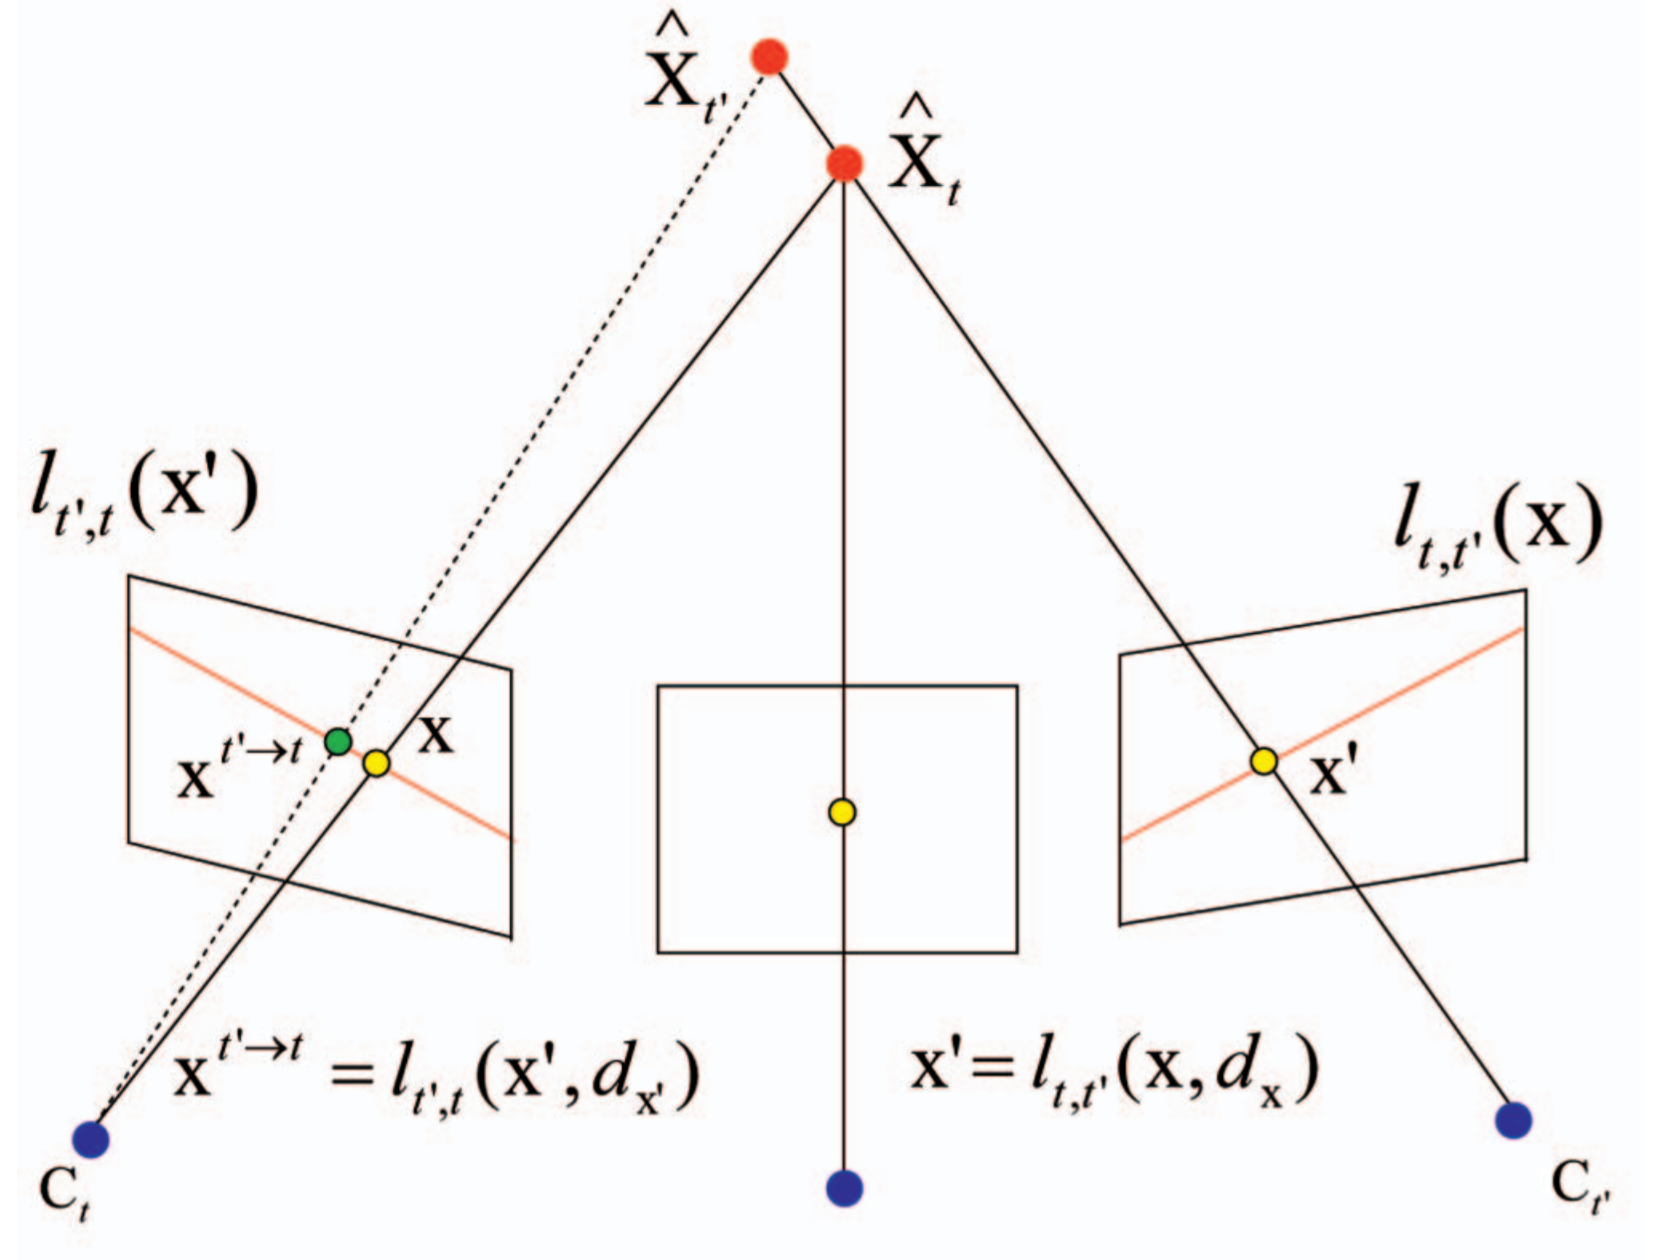
\includegraphics[width=.75\textwidth]{conjugate_pixel.png} %{CS0031}
	\caption{}
\end{figure}

%%%----------------------------------------------------------
\MakeBibliography[nosplit]
%%%----------------------------------------------------------


\end{document}
